\chapter{Mise en oeuvre de la solution}

\label{sec:realisation}

\begin{fquote}
Dans ce chapitre, on va présenter les outils utilisés pour la mise en oeuvre de la solution PIM ainsi qu’un aperçu des différentes vues et interfaces de cette solution.
\end{fquote}

\clearpage

\section{Introduction :}

Une des étapes de la vie d’un projet, aussi importante que la conception, est l’implémentation.

\medskip

Cette étape constitue la phase d’achèvement et d’aboutissement du projet. Pour accomplir cette tâche avec succès il faut savoir utiliser les outils adéquats et nécessaires. Ce choix d’outils peut influencer la qualité du produit obtenu et donc nécessite une attention particulière et doit se baser sur les besoins du projet et le résultat escomptés.

\medskip

Ce chapitre présente l’environnement technique du travail ainsi que le choix pris en matière d’environnement logiciel. 

\section{Environnement de travail : Outils et technologies utilisées }
\subsection{Environnement matériel}
Pour la réalisation de ce projet nous avons utilisé le matériel suivant :

\begin{table}[h]
	

	\begin{center}
		\begin{tabular}{>{\begin{bf} } c <{\end{bf}}ccc}
			
			\rowcolor{-blue!20!red}Pc portable & \begin{bf}Asus VivoBook 15 x510UA \end{bf} & \begin{bf}HP Notebook 15\end{bf} & \\
			
			RAM & 8 GO & 8 GO& \\
			Microprocesseur & Intel(R)Core(TM)i5-8250U &Intel(R)Core(TM)i3-45005U & \\
			Disque dur & 240 GB SSD & 240 GB SSD& \\
			System d'exploitation & Windows 10 Profissional & Windows 10 Profissional& \\
			
			
			
			
			
		\end{tabular}
	\end{center}
	\caption{Description de la machine de développement}
	\label{Description de la machine de développement}
\end{table}



\subsection{Environnement logiciel}

\subsubsection{Outils de développement et modélisation :}
Les principaux outils qui ont contribué à la qualité du développement sont :

\begin{itemize}
	\item[$\bullet$] \textbf{Visual Studio Code : Environnement de développement intégré } \footnote{Visual Studio Code : est un éditeur de code extensible développé par Microsoft pour Windows, Linux et macOS1.}est un éditeur de code multiplateforme édité par Microsoft. Ce outil destiné aux développeurs supporte plusieurs dizaines de langages de programmation comme le HTML, C++, PHP, Javascript, Markdown, CSS, etc. \cite{wiki:Visual_Studio_Code}
\begin{figure}[ht]
	\centering
	
\includegraphics[width=3cm,height=2.5cm]{VisualStudioCode.png}
	\caption{Logo Visual code studio.}
	\label{fig:VisualStudioCode }
\end{figure}
\FloatBarrier

\medskip

\item[$\bullet$] \textbf{StarUML : Outils de modélisation} 
est un logiciel de modélisation UML (Unified Modeling Language) open source qui peut remplacer dans bien des situations des logiciels commerciaux et coûteux comme Rational Rose\footnote{Présentation sur le site web d’IBM France :
\url{http://ibm.co/1hre0xd } } ou Together\footnote{Présentation en anglais sur le site web de Borland : \url{http://www.borland.com/products/Together/ }}
. Étant simple d’utilisation, nécessitant peu de
ressources système, supportant UML 2, ce logiciel constitue une excellente option pour une familiarisation à la modélisation. Cependant, seule une version Windows est disponible . \cite{wiki:StarUML} 
	\begin{figure}[ht]
		\centering
		
\includegraphics[width=7cm,height=5cm]{maxresdefault.jpg}
		\caption{Logo StarUML.}
		\label{fig:StarUML }
	\end{figure}
	\FloatBarrier
    \medskip


\item[$\bullet$] \textbf{MySQL \footnote{ \url{https://www.mysql.com/fr/} }} 
MySQL(My Structured Query Langage-Langage de requêtes structuré) est un système de
gestion de bases de données relationnelles dédiées Open source. Il est très rapide, fiable et facile à utiliser et gratuit.il a été développé à l’origine pour gérer des très grandes bases de données beaucoup plus rapidement que des solutions déjà établies. Il offre un ensemble de fonctionnalités large et riche. Sa rapidité et sa sécurisation en font un outil idéal pour les applications internet .\cite{wiki:MySQL} 
\begin{figure}[ht]
	\centering
	
\includegraphics[width=7cm,height=5cm]{mysql.jpg}
	\caption{Logo MySQL.}
	\label{fig:Logo MySQL }
\end{figure}
\FloatBarrier
\medskip
















   \item[$\bullet$] \textbf{ XAMPP \footnote{XAMPP est l'environnement de développement PHP le plus populaire \url{https://www.apachefriends.org/fr/index.html} }} est un ensemble de logiciels permettant de mettre
    en place facilement un serveur Web
    confidentiel, un serveur FTP et un serveur de messagerie
    électronique. Il s’agit d’une distribution de logiciels libres (X
    (cross) Apache MariaDB Perl PHP) offrant une bonne
    souplesse d'utilisation , réputée pour son installation
    simple et rapide. Ainsi, il est à la portée d’un grand nombre de
    personnes puisqu'il ne requiert pas de connaissances
    particulières et fonctionne, de plus, sur les systèmes
    d'exploitation les plus répandus.
 \cite{wiki:XAMPP} 
    \begin{figure}[ht]
    	\centering
    	
\includegraphics[width=7cm,height=5cm]{xampplogo.jpg}
    	\caption{Logo XAMPP.}
    	\label{fig:xampp logo}
    \end{figure}
    \FloatBarrier
    
        \medskip
    
   \item[$\bullet$] \textbf{Apache Tomcat\footnote{\url{http://tomcat.apache.org/}} :} C'est un conteneur web libre de servlets et JSP Java EE. Issu du projet Jakarta. Il incorpore également un serveur HTTP\cite{wiki:tomcat}.
    
 c’est un des nombreux projets de l’Apache Software Foundation. Il implémente les spécifications des servlets et des JSP du Java Community Process, et paramétrable par des fichiers XML et des propriétés, et inclut des outils pour la configuration et la gestion.
 
  \begin{figure}[ht]
 	\centering
 	
\includegraphics[width=7cm,height=5cm]{unnamed.jpg}
 	\caption{Logo Apache Tomcat.}
 	\label{fig:Apache Tomcat}
 \end{figure}
 \FloatBarrier
\medskip
\end{itemize}


\subsubsection{Langages de programmation :}

\begin{itemize}
	\item[$\bullet$] \textbf{HTML 5 :} 	
 signifie « HyperText Markup Language » qu’on peut traduire par « langage de
balises pour l’hypertexte ». Il est utilisé afin de créer et de représenter le contenu d’une
page web et sa structure. D’autres technologies sont utilisées avec HTML pour décrire la
présentation d’une page (CSS) et/ou ses fonctionnalités interactives (JavaScript).
HTML fonctionne grâce à des « balises » qui sont insérées au sein d’un texte normal.
Chacune de ces balises indique la signification de telle ou telle portion de texte dans
le site. On parle d’« hypertexte » en référence aux liens qui connectent les pages web
entre elles. C’est la mécanique originelle du « World Wide Web » que nous connaissons
aujourd’hui. En écrivant et publiant des pages web, vous devenez un acteur du Web dès
que votre site est accessible en ligne.\cite{wiki:Hypertext_Markup_Language}
	\begin{figure}[ht]
		\centering
		
\includegraphics[width=3cm,height=2.5cm]{HTML5.png}
		\caption{Logo HTML.}
		\label{fig:HTML5 }
	\end{figure}
	\FloatBarrier	
	\medskip
	

		\item[$\bullet$] \textbf{CSS4 :} 
Depuis les spécifications des feuilles de style en cascade CSS3 qui introduit le passage à la modularisation, chaque module évolue indépendamment des autres.

Certains modules commencent avec leur propre version et contrôle de niveau (exemple : CSS Grid).

Les mises à jour actuelles des CSS sont appelées CSS4.\cite{wiki:Feuilles_de_style_en_cascade}
		\begin{figure}[ht]
			\centering
			
\includegraphics[width=3cm,height=2.5cm]{css.png}
			\caption{Logo CSS4.}
			\label{fig:CSS4 }
		\end{figure}
		\FloatBarrier
		
		\medskip
		
		
	\item[$\bullet$] \textbf{Bootstrap 4 \footnote{Bootstrap : C’est un ensemble de fichiers (html, css, et javascript) qui va servir de bases pour la création de pages web.}:} 
Bootstrap est le framework HTML, CSS et JS le plus populaire au monde pour la création de pages web interactives et responsives.

Il est entièrement gratuit. Des millions de sites sur le Web sont réalisés avec Bootstrap.. Apprenez vous aussi à l’utiliser (dernière version 4).\cite{wiki:Bootstrap_(front-end_framework)}
\begin{figure}[ht]
	\centering
	
\includegraphics[width=3cm,height=2.5cm]{bootstrap.png}
	\caption{Logo Bootstrap.}
	\label{fig:Logo bootstrap }
\end{figure}
\FloatBarrier

\medskip	



\item[$\bullet$] \textbf{ GIT et GitHub : Outils de versioning}

	\begin{itemize}	
	\item[$\star$] GIT :  C'est un logiciel libre de gestion de versions, créé par Linus Torvalds(le créateur du noyau Linux), c’est un outil bas niveau, qui se veut simple et très performant, dont la principale tâche est de gérer l’évolution du contenu d’une arborescence. Il fonctionne en mode distribué avec un serveur distant\cite{wiki:git}.
	\item[$\star$] GitHub \footnote{GitHub : est un service en ligne qui permet d'héberger ses repositories de code.}: est une société à but lucratif qui offre un service d’hébergement de référentiel Git basé sur le cloud. Essentiellement, il est beaucoup plus facile pour les individus et les équipes d’utiliser Git pour le contrôle de version et la collaboration.
	
	L’interface de GitHub est suffisamment conviviale pour que même les codeurs débutants puissent profiter de Git. Sans GitHub, l’utilisation de Git nécessite généralement un peu plus de connaissances techniques et l’utilisation de la ligne de commande.

\end{itemize}



\begin{figure}[ht]
	\centering
	
\includegraphics[width=6cm,height=4cm]{git.jpg}
	\caption{Logo GIT et GitHub.}
	\label{fig:GIT et GitHub }
\end{figure}
\FloatBarrier

\medskip




	\item[$\bullet$] \textbf{ php 7.1.3 :} 
HyperText Preprocessor, plus connu sous
son sigle PHP, est un langage de programmation
principalement utilisé pour produire des pages Web
dynamiques via un serveur HTTP, mais pouvant
également fonctionner comme n'importe quel
langage interprété de façon locale. PHP est un
langage impératif orienté-objet.\cite{wiki:PHP}
\begin{figure}[ht]
	\centering
	
\includegraphics[width=3cm,height=2.5cm]{php.png}
	\caption{Logo php 7.1.3.}
	\label{fig:Logo php }
\end{figure}
\FloatBarrier





	\item[$\bullet$] \textbf{ Laravel 5.7 :\footnote{ \url{https://laravel.sillo.org/laravel-5-7-par-la-pratique-introduction/} }} 
Laravel est un framework web open-source écrit en PHP1 respectant le principe modèle-vue-contrôleur et entièrement développé en programmation orientée objet. Laravel est distribué sous licence MIT, avec ses sources hébergées sur GitHub.

\cite{wiki:Laravel}
\begin{figure}[ht]
	\centering
	
\includegraphics[width=3cm,height=2.5cm]{laravel.png}
	\caption{Logo Laravel.}
	\label{fig:Laravel }
\end{figure}
\FloatBarrier

\medskip

	\item[$\bullet$] \textbf{ InfyOm Laravel:\footnote{ \url{https://labs.infyom.com/laravelgenerator/docs/7.0/introduction} }} 
 Generator qui prend 
en charge Laravel API, Scaffold, CRUD,
Test Case, Swagger Docs et Auth generator.
L'utilisation de ce générateur est  générer des cas de test Laravel, 
des documents Swagger, des annotations Swagger, de la documentation API (API Docs), CRUD à partir d'une table existante et un Scaffoldà partir d'une base de données existante.
\cite{wiki:Laravel}
\begin{figure}[ht]
	\centering
	
\includegraphics[width=5cm,height=3cm]{Infyom.png}
	\caption{Logo Infyom.}
	\label{fig:Infyom }
\end{figure}
\FloatBarrier

\medskip


\end{itemize}
\section{Outils de rédaction du rapport:}
\begin{itemize}

	\item[$\bullet$] \textbf{ LaTeX : \footnote{ Un éditeur LaTeX en ligne facile à utiliser\url{https://fr.overleaf.com} }} 
Nous avons utilisé LaTeX pour la rédaction du rapport, LaTex est un système de composition
de haute qualité. Il comprend des fonctionnalités conçues pour la production de documentation
technique et scientifique. LaTeX est la norme de facto pour la communication et la publication de
documents scientifiques.\footnote{ TeXstudio (anciennement TeXMakerX) est un environnement de développement intégré (IDE) très puissant pour écrire des documents LaTeX en format PDF ou autre, qui s’affichent de la même manière quelque soit le système d’exploitation.\url{https://sourceforge.net/projects/texstudio/} }\cite{wiki:PHP}
\begin{figure}[ht]
	\centering
	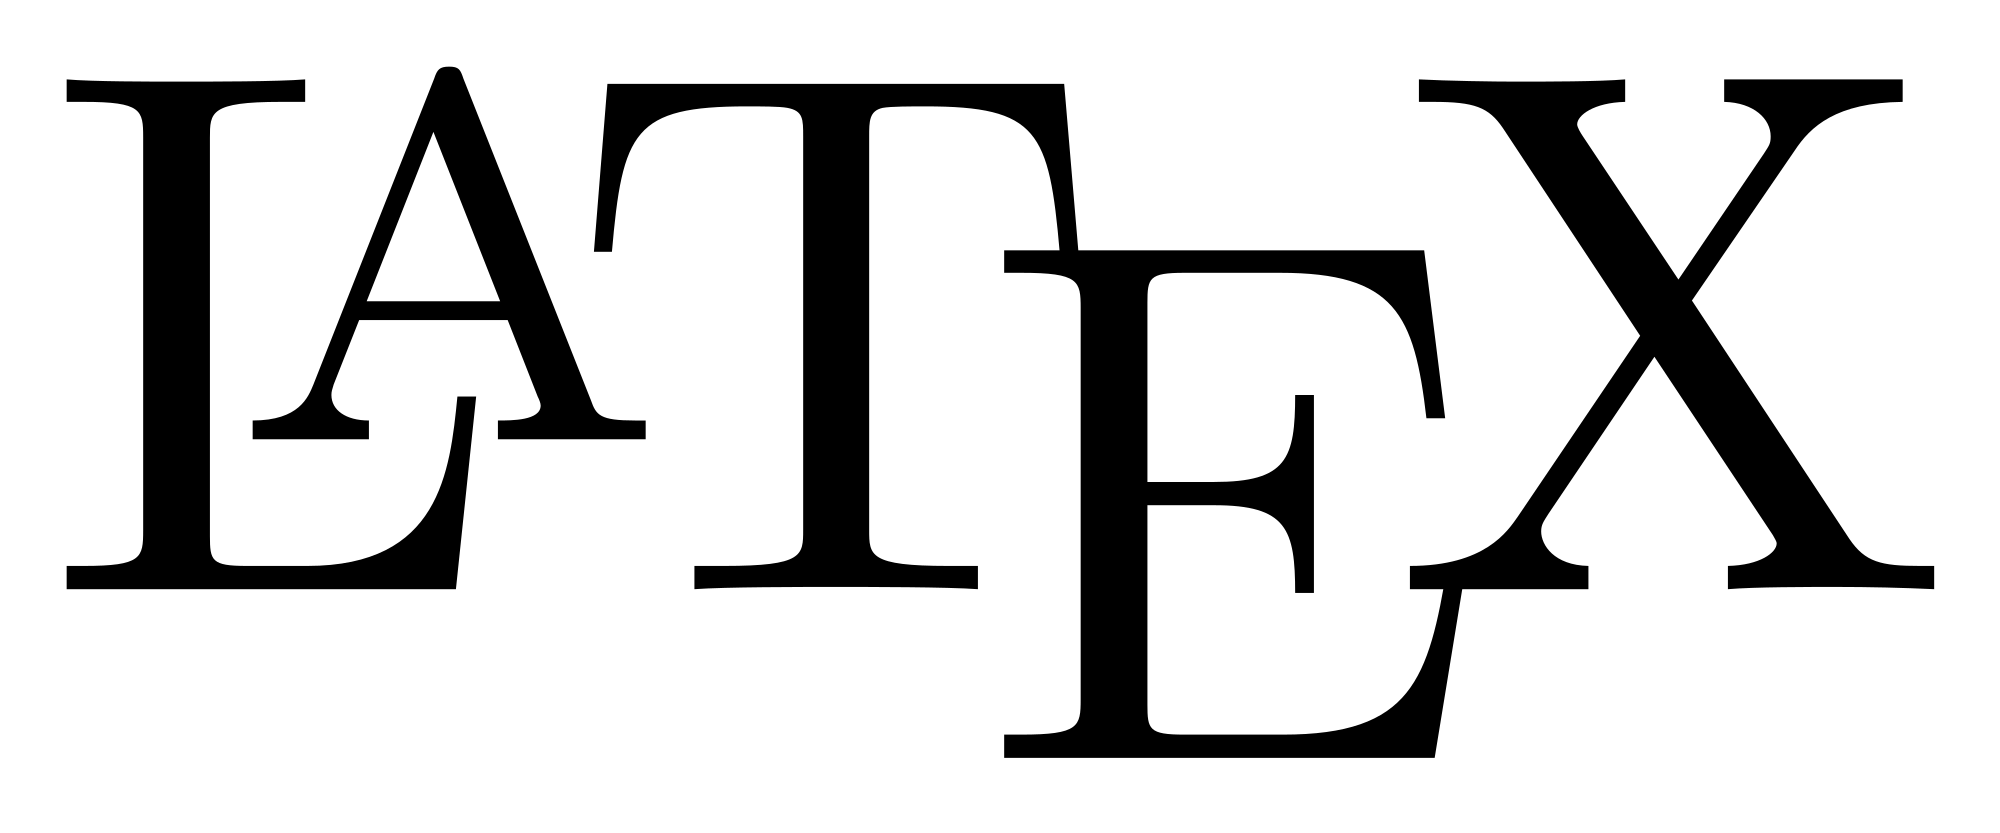
\includegraphics[width=3cm,height=2.5cm]{LaTeX.png}
	\caption{Logo LaTeX}
	\label{fig:LaTeX }
\end{figure}
\FloatBarrier

\medskip


\end{itemize}

















\clearpage





 


\section{Conclusion}
Dans ce chapitre, on a présenté la réalisation qu'on a effectué, l’environnement de développement, les outils et technologies utilisés dans le projet ainsi qu'une description détaillée des différentes interfaces utilisateur de la plate-forme.


